\section{Model Sztucznej Inteligencji}
\label{sec:model_ai}

\subsection{Charakterystyka problemu segmentacji semantycznej}

Model sztucznej inteligencji stanowiący podstawę niniejszego projektu został zaprojektowany do rozwiązywania zadania \textbf{segmentacji semantycznej obrazów wodomierzy}. Celem segmentacji jest przypisanie każdemu pikselowi obrazu etykiety określającej jego przynależność do jednej z wyróżnionych klas, w szczególności obszaru licznika, tarczy oraz tła.

Problem ten ma istotne znaczenie praktyczne w kontekście automatyzacji odczytu wskazań wodomierzy, gdzie poprawne wydzielenie obszaru licznika stanowi warunek konieczny dla dalszych etapów przetwarzania obrazu, takich jak rozpoznawanie cyfr lub analiza wskazań mechanicznych. W przeciwieństwie do klasycznej klasyfikacji obrazów, segmentacja semantyczna wymaga zachowania informacji przestrzennej oraz precyzyjnego odwzorowania granic obiektów, co znacząco zwiększa złożoność problemu.

Dodatkowym wyzwaniem są zmienne warunki akwizycji danych, obejmujące różnice w oświetleniu, kącie wykonania zdjęcia, jakości obrazu oraz stopniu zabrudzenia lub zużycia urządzeń pomiarowych. Czynniki te powodują, że klasyczne algorytmy przetwarzania obrazu okazują się niewystarczające, co uzasadnia zastosowanie metod opartych na uczeniu głębokim.

\begin{figure}[H]
  \centering
  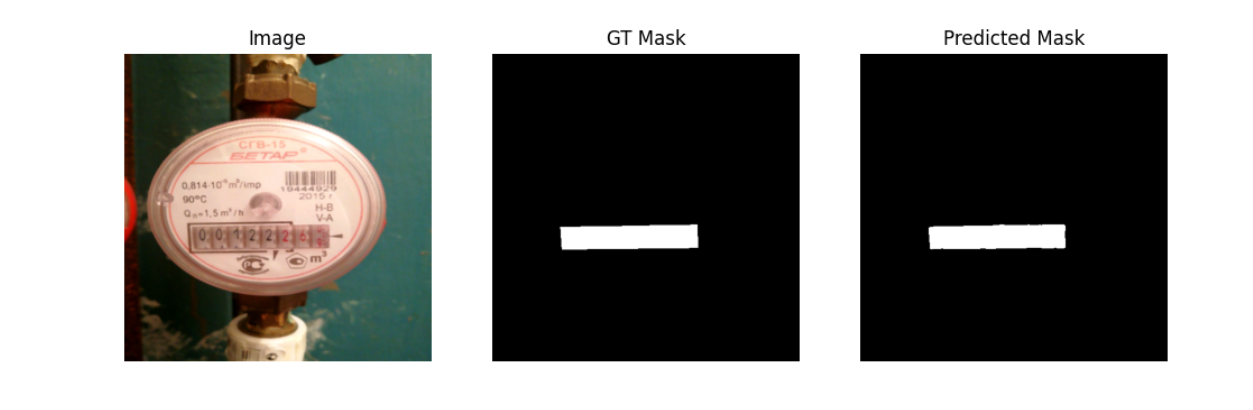
\includegraphics[width=\textwidth]{img/04_model_sztucznej_inteligencji/Example_Prediction.png}
  \caption{Przykład predykcji modelu segmentacji semantycznej}
  \label{fig:example_prediction}
\end{figure}

\subsection{Architektura modelu}

W projekcie wykorzystano konwolucyjną sieć neuronową opartą na architekturze \textbf{U-Net}, powszechnie stosowaną w zadaniach segmentacji semantycznej obrazów. Architektura ta charakteryzuje się symetryczną budową typu encoder--decoder, umożliwiającą jednoczesne wydobywanie cech semantycznych oraz zachowanie informacji przestrzennej.

Część kodująca (encoder) odpowiada za stopniowe przekształcanie obrazu wejściowego do reprezentacji o coraz wyższym poziomie abstrakcji poprzez sekwencję operacji konwolucji oraz redukcji rozdzielczości. Część dekodująca (decoder) realizuje proces rekonstrukcji obrazu wyjściowego, przywracając jego pierwotną rozdzielczość i generując maskę segmentacyjną.

Kluczowym elementem architektury są tzw. \textit{skip connections}, umożliwiające bezpośrednie przekazywanie map cech pomiędzy odpowiadającymi sobie poziomami enkodera i dekodera. Mechanizm ten pozwala ograniczyć utratę informacji lokalnej oraz poprawić jakość segmentacji, szczególnie w obszarach granicznych pomiędzy klasami.

Zastosowana implementacja architektury U-Net została dostosowana do specyfiki problemu, w tym rozdzielczości obrazów wejściowych oraz liczby klas segmentacyjnych. Model generuje maskę wyjściową o tej samej rozdzielczości co obraz wejściowy, co ułatwia dalsze etapy przetwarzania oraz ocenę jakości predykcji.

\begin{figure}[H]
  \centering
  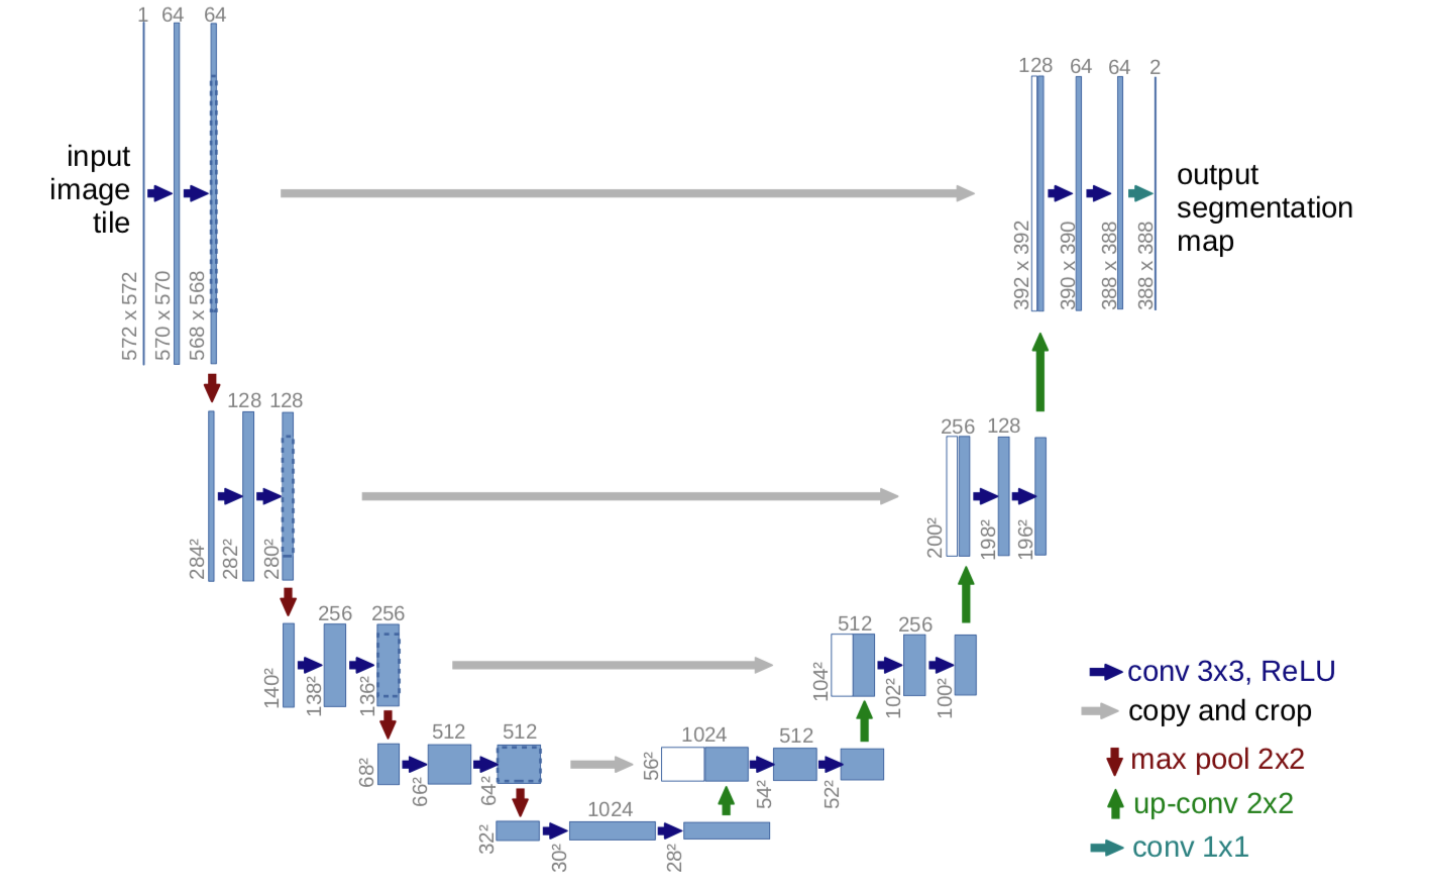
\includegraphics[width=\textwidth]{img/04_model_sztucznej_inteligencji/U-NET.png}
  \caption{Schemat architektury U-Net \cite{unet_segmentacja_blog}}
  \label{fig:unet_architecture}
\end{figure}

\subsection{Dane treningowe i przygotowanie zbioru danych}

Model został wytrenowany na zbiorze danych składającym się z obrazów wodomierzy oraz odpowiadających im masek. Każda próbka zawiera obraz wejściowy w postaci fotografii oraz maskę określającą przynależność poszczególnych pikseli do zdefiniowanych klas.

Proces przygotowania danych obejmował normalizację wartości pikseli, standaryzację rozdzielczości obrazów oraz podział zbioru danych na część treningową, walidacyjną i testową. W celu zwiększenia odporności modelu na zmienność danych wejściowych zastosowano techniki augmentacji danych, takie jak losowe obroty, skalowanie, przesunięcia oraz modyfikacje jasności i kontrastu.

Zastosowanie augmentacji pozwala ograniczyć ryzyko przeuczenia modelu oraz poprawić jego zdolność do generalizacji na dane niewidziane w procesie uczenia. Istotnym aspektem projektu jest fakt, że zbiór danych oraz jego kolejne wersje podlegają wersjonowaniu, co umożliwia jednoznaczne powiązanie konkretnej wersji modelu z użytymi danymi treningowymi.

Zbiór danych wykorzystany w projekcie pochodzi z platformy Kaggle \cite{kaggle_water_meters}.

\subsection{Proces uczenia i metryki jakości}

Proces uczenia modelu realizowany jest w sposób nadzorowany, z wykorzystaniem funkcji straty dostosowanej do problemu segmentacji semantycznej. Jako główne metryki oceny jakości modelu zastosowano \textbf{współczynnik Dice} oraz \textbf{Intersection over Union (IoU)}, które są standardowymi miarami stosowanymi w zadaniach segmentacyjnych.

Współczynnik Dice umożliwia ocenę stopnia pokrycia obszaru przewidywanego przez model z obszarem referencyjnym, natomiast IoU mierzy stosunek części wspólnej obu obszarów do ich sumy. Zastosowanie obu metryk pozwala na bardziej kompleksową ocenę jakości predykcji, szczególnie w przypadku niezbalansowanych klas.

Proces uczenia realizowany jest iteracyjnie, z wykorzystaniem zbioru walidacyjnego do monitorowania jakości modelu oraz ograniczania zjawiska przeuczenia. Najlepsza wersja modelu, zgodnie z przyjętymi kryteriami jakości, zapisywana jest jako artefakt i przekazywana do dalszych etapów zautomatyzowanego pipeline’u CI/CD.

\subsection{Model jako artefakt w procesie CI/CD}

W kontekście niniejszej pracy model sztucznej inteligencji traktowany jest jako pełnoprawny artefakt inżynierski, podlegający wersjonowaniu, testowaniu oraz kontrolowanemu wdrażaniu. Każda wersja modelu jest jednoznacznie powiązana z wersją kodu źródłowego, zestawem danych treningowych, konfiguracją hiperparametrów oraz uzyskanymi metrykami jakości.

Takie podejście umożliwia pełną reprodukowalność wyników oraz stanowi podstawę do dalszej analizy porównawczej pomiędzy podejściem manualnym a zautomatyzowanym procesem CI/CD. Szczegółowa analiza wpływu automatyzacji na jakość, stabilność oraz koszty utrzymania modeli sztucznej inteligencji zostanie przedstawiona w kolejnych rozdziałach pracy.

\begin{figure}[H]
  \centering
  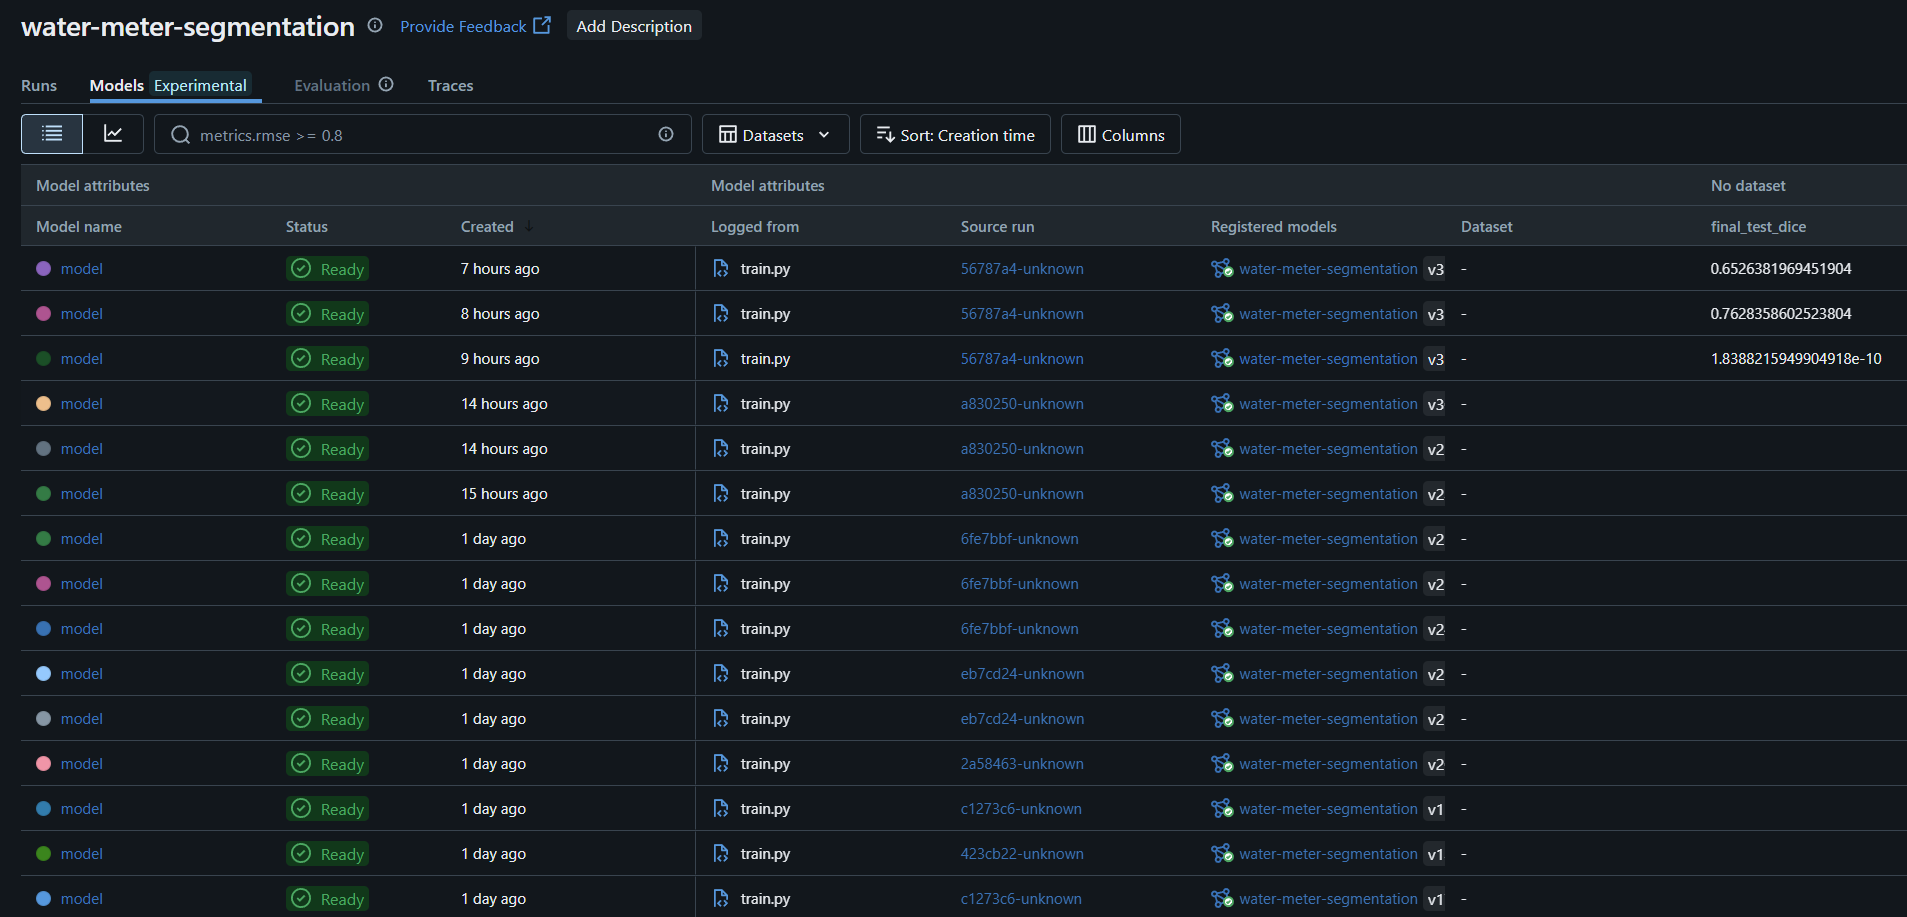
\includegraphics[width=\textwidth]{img/04_model_sztucznej_inteligencji/mlflow_versions.png}
  \caption{Wersjonowanie modeli w rejestrze MLflow}
  \label{fig:mlflow_versions}
\end{figure}
